\documentclass[11pt]{beamer}
\usetheme{Madrid}
\usepackage[utf8]{inputenc}
\usepackage{amsmath, amssymb, amsfonts, amsthm}
\usepackage{xcolor}

\usepackage{tikz-cd}

\author[\texttt{sebastiano.tronto@uni.lu}]{Sebastiano Tronto}
\title{Presentations in LaTeX with Beamer}
\logo{
\includegraphics[scale=0.1]{img/unilu.jpg}} 
%\institute{University of Luxembourg} 

\newcommand{\bs}{\textbackslash}

\date{2021-03-26} 

\begin{document}

\begin{frame}
  \titlepage
\end{frame}

\begin{frame}{Why presentation with LaTeX?}
  Pros:

  \vspace{0.2cm}
  \begin{itemize}
    \item Easy to include formulas and theorems
    \item Portability: \texttt{pdf} = \textbf{portable} document format
    \item Very fast to get ``good enough'' results (subjective)
  \end{itemize}

  \vspace{0.5cm}
  Cons:

  \vspace{0.2cm}
  \begin{itemize}
    \item Advanced animations not possible with pdf
    \item Lack of other presentation-specific features
  \end{itemize}
\end{frame}

\begin{frame}{Structure of a Beamer document}
  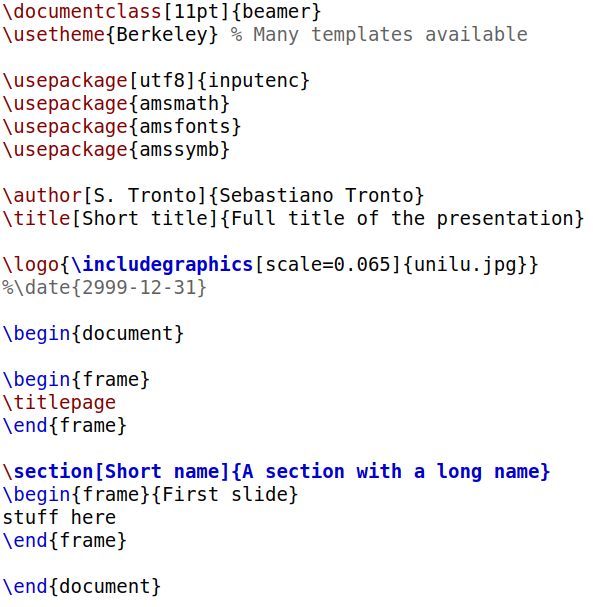
\includegraphics[scale=0.35]{img/beamer.png}
\end{frame}

\begin{frame}{The \texttt{frame} environment}
  \texttt{\bs begin\{frame\}[options]\{Title\} \,\dots\, \bs end\{frame\}}

  \vspace{0.5cm}
  Useful options:
  \begin{itemize}
    \item \texttt{plain}: no bars on bottom or side
    \item \texttt{shrink}: content is shrunk to fit in the slide
    \item \texttt{fragile}: when you have \texttt{tikzpicture},
          \texttt{listings} or similar 
  \end{itemize}
\end{frame}

\begin{frame}{Basic animations}
  \begin{itemize}
    \item \texttt{\bs pause} for a simple break

    \vspace{0.3cm}
    \item \texttt{\bs only<start-(end)>\{\emph{stuff}\}} to show
          \emph{\texttt{stuff}} only on some slides
          
          Shortcut for lists: \texttt{\bs item<\dots>} or
          \texttt{\bs begin\{itemize\}[<+->]}

    \vspace{0.3cm}
    \item Optional:
          \texttt{\bs setbeamercovered\{transparent\}} (see end of slides)

    \vspace{0.3cm}
    \item \texttt{\bs uncover<\dots>} does not take space when invisible
  \end{itemize}
\end{frame}

\begin{frame}{Theorems and lists}
  \begin{theorem} This is a Theorem \end{theorem}
  \begin{proof} With proof \end{proof}
  
  \begin{itemize}
    \item \texttt{theorem}, \texttt{proof} and \texttt{definition} already
          included with beamer.
    \item Define new theorems as usual (they get a box automatically)
  \end{itemize}
\end{frame}

\begin{frame}[fragile]{Custom blocks}

  {
    \setbeamercolor{block title}{fg=blue,bg=green}
    \setbeamercolor{block body}{fg=black,bg=pink!50}
    \begin{block}{A custom block, with ugly colors}
      \begin{verbatim}
{
    \setbeamercolor{block title}{fg=blue,bg=green}
    \setbeamercolor{block body}{fg=black,bg=pink!50}
    
    \begin{block}{A custom block, with ugly colors}
        ...
    \end{block}
}
      \end{verbatim}
    \end{block}
  }
\end{frame}


\begin{frame}{Multiple columns}
  \begin{columns}
  \column{0.3\textwidth}
    \texttt{\bs begin\{columns\}}

    \texttt{\qquad\bs column\{\emph{width}\}}

    \texttt{\qquad(stuff)}

    \texttt{\qquad\bs column\{\emph{width}\}}

    \texttt{\qquad(more stuff)}

    \texttt{\qquad\qquad\vdots}

    \texttt{\bs end\{columns\}}
  \column{0.7\textwidth}
    \begin{itemize}
      \item \texttt{\emph{width}} is a length (example:
            \texttt{0.7\bs textwidth})
      \item Example: picture on the left, text on the right
      \item Not specific to Beamer
      \item Alternative: \texttt{tabular}
    \end{itemize}
  \end{columns}

\end{frame}

\begin{frame}{Some advice}
  \begin{itemize}
    \item Do not prepare too many slides (1-2 minutes per slide)
    \item Do not write too much in each slide (split if necessary)
    \item Pictures and \texttt{itemize}s are great, sentences are not
    \item Animations are ok (but are they worth the effort?)
  \end{itemize}
\end{frame}

\begin{frame}{Examples}
  Three examples will follow:
  \begin{itemize}
    \item A horrible slide
    \item A better slide with the same content
    \item A better better slide that took a little more time to write
  \end{itemize}
\end{frame}

\begin{frame}{Diophantine equations (bad)}
  Diophantine equations are a very old problem, dating back to Diophantus of
  Alexandria (III century A.D.).

  Despite this, they are still today a very hard problem, and there is
  no general method or algorithm to solve them.

  A notable example is \emph{Fermat's Last Theorem}, stated for the first time
  in 1637 but proved to be true only in 1995, after more than 350 years!
\end{frame}


\begin{frame}{Diophantine Equations (better)}
  \begin{itemize}
    \item Very old problem
    
    \vspace{0.3cm}
    \item Very simple formulation, but very hard to solve!
    
    \vspace{0.3cm}
    \item ``Fermat's Last Theorem'': stated in 1637 - proved in 1995
  \end{itemize}
\end{frame}

\setbeamercovered{transparent}
\begin{frame}{Diophantine Equations (better better)}
  \begin{columns}
  \column{0.45\textwidth}
    \begin{figure}
      \begin{center}
        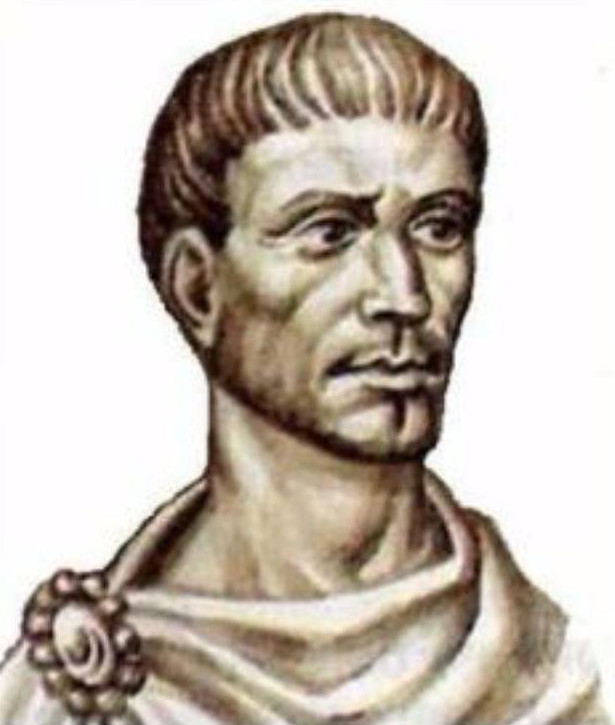
\includegraphics[scale=0.2]{img/diophantus.jpg}
        {\footnotesize Diophantus of Alexandria\\ (III century A.D.)}
      \end{center}
    \end{figure}
  \column{0.55\textwidth}
    \begin{itemize}
      \item<1-> Very old problem
      \item<2-> Very simple formulation, but very hard to solve!
      \item<3-> \emph{Fermat's Last Theorem}: stated in 1637 - proved in 1995
    \end{itemize}
  \end{columns}
\end{frame}


\end{document}
